% Load preamble
\documentclass[../main.tex]{subfiles}

\begin{document}
	\subsection{Príklad druhý}
	Majme systém, ktorý je určený stavovým opisom \cref{eqn:svlv2vrov}. Bloková schéma systému je na \cref{fig:svlvv2schfig}.
	\begin{equation}
		\begin{aligned}
		\dot{x_1} &= x_2 - x_1^3\\
		\dot{x_2} &= 2x_3^2 + (x_1^2+1)u \\
		\dot{x_3} &= x_1 + x_2^3 - 3x_3^3 \\
		y &= x_1
		\end{aligned}
		\label{eqn:svlv2vrov}
	\end{equation}
	\begin{figure}[h!]
		\centering
		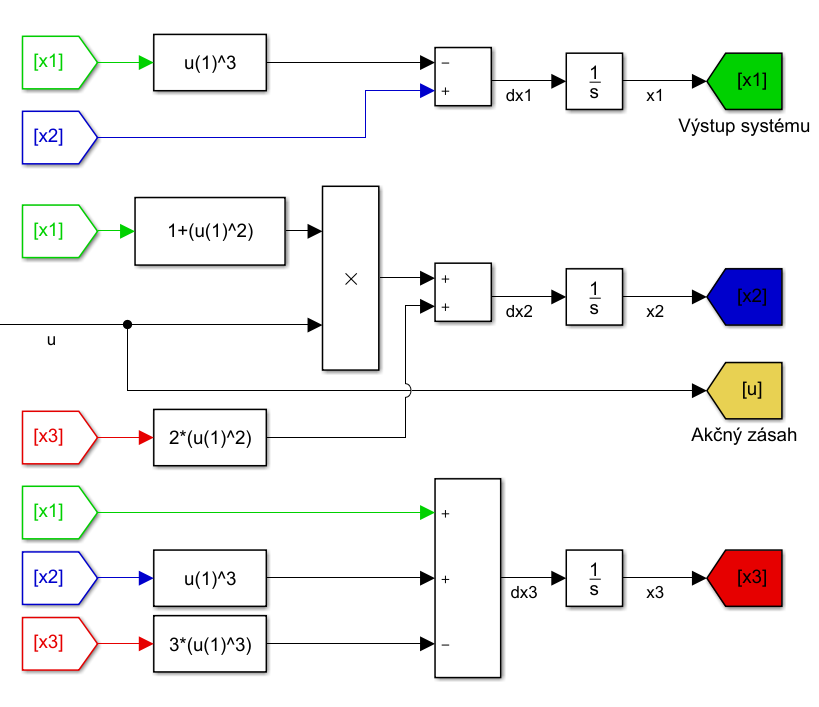
\includegraphics[width=0.8\linewidth]{sysPr2}
		\caption{Bloková schéma systému z \cref{eqn:svlv2vrov}}
		\label{fig:svlvv2schfig}
	\end{figure}
	\subsubsection{Návrh riadenia}
	Teraz overíme, že bod  $x_1 = x_2 = x_3 = 0 $, je rovnovažný bodom systému. Systém sa nachádza v rovnováhe, keď časové derivácie všetkých stavových premenných sú nulové. 
	\begin{equation}
		\begin{aligned}
		\dot{x_1}|_{x_1 = x_2 = x_3 = 0} &= 0 - 0 = 0 \\
		\dot{x_2}|_{x_1 = x_2 = x_3 = 0} &= 0    = 0 \\
		\dot{x_3}|_{x_1 = x_2 = x_3 = 0} &= 0 + 0 - 0 = 0 \\
		\end{aligned}
		\label{eqn:svlvvPr2OvereniePB}
	\end{equation}
	
		Ako vidíme v bode $x_1 = x_2 = x_3 = 0 $ sú derivácie stavových premenných v čase nulové, teda bod $x_1 = x_2 = x_3 = 0 $ je rovnovážny bod systému.
	
	Našim cieľom je riadiť tento systém tak, aby výstup dosiahol žiadanú hodnotu $r$.
	
	Aplikujeme nelineárne riadenie, opäť navrhnuté metódou vstupno výstupnej spätnoväzobnej linearizácie použitú aj v predchádzajúcom príklade. 
	
	Rovnako ako v predchádzajúcom prípade je prvým krokom derivovanie vzťahu pre výstup systému $y$. Tento vzťah je potrebné derivovať pokiaľ sa v ňom neobjaví vstupný signál $u$. 

 	\begin{equation}
	\begin{aligned}
	y &= x_1 \\ 
	\implies \dot{y}  &= \dot{x_1} =  x_2 - x_1^3 \\
	\implies \ddot{y} &= \dot{x_2} - 3x_1^2\dot{x_1} \\
	\implies \ddot{y} &= 2x_3^2 + (x_1^2 + 1)u - 3x_1^2x_2 + 3x_1^5 \\
	&= 2x_3^2 - 3x_1^2x_2 + 3x_1^5 + (x_1^2 + 1)u\\
	\end{aligned}
	\label{eqn:svlvvPr2DerVys}
	\end{equation}
	Pre zjednodušenie do budúcna upravme výslednú \cref{eqn:svlvvPr2DerVys} nasledovne:
	 \begin{equation}
	\begin{aligned}
	\ddot{y} &= f(x_1,x_2,x_3) + (x_1^2 + 1)u \\
	f(x_1,x_2,x_3) &= 2x_3^2 - 3x_1^2x_2 + 3x_1^5\\
	\end{aligned}
	\label{eqn:svlvvPr2DerUp}
	\end{equation}
	
	Ak zvolíme vstup do systému, tak ako je v \cref{eqn:svlvvPr2ZakLin}, po dosadení dostaneme \cref{eqn:svlvvPr2Dos}. Voľba takéhoto zákona je nazývaná zákonom linearizácie, pre vstup $u$ do systému.
	\begin{equation}
	u = \frac{v - f(x_1,x_2,x_3)}{x_1^2 + 1}
	\label{eqn:svlvvPr2ZakLin}
	\end{equation}
	\begin{equation}
	\begin{aligned}
	\ddot{y} &= 2x_3^2 - 3x_1^2x_2 + 3x_1^5 + (x_1^2 + 1)\frac{v - f(x_1,x_2,x_3)}{x_1^2 + 1} \\
	\ddot{y} &=v  \\ 
	\end{aligned}
	\label{eqn:svlvvPr2Dos}
	\end{equation}
	
	Posledný krok. Ak si zvolíme $v$ podľa \cref{eqn:svlvvPr2ZakRiad}, tak dostávame rovnicu pre dynamiku odchýlky \cref{eqn:svlvvPr2DynOdch}. Ak zvolíme koeficienty $k$ všetky kladné, dynamika odchýlky bude vždy stabilná a bude konvergovať k 0. Voľba tohto zákona, pre $v$, povedzme zákona riadenia linearizovaného systému. Pozn. $e = (r - y)$
	\begin{equation}
	\begin{aligned}
	v &= \ddot{r} - k_1 (\dot{y} - \dot{r}) - k_2(y-r)\\
	\end{aligned}
	\label{eqn:svlvvPr2ZakRiad}
	\end{equation}
	\begin{equation}
	\begin{aligned}
	v &= \ddot{r}  +k_1 \dot{e} + k_2 e \\
	\implies \ddot{y} &= \ddot{r}  +k_1 \dot{e} + k_2 e \\
	\implies 0 &= \ddot{e}  + k_1 \dot{e} + k_2 e \\	 
	\end{aligned}
	\label{eqn:svlvvPr2DynOdch}
	\end{equation}
	
	Máme navrhnutý lineárny regulátor. Kompletný systém vidíme na \cref{fig:svlvvPr2All}.  Výsledky zo simulácie, pre niekoľko žiadaných úrovní výstupu je na \cref{fig:svlvvPr2Vys}.
	\begin{figure}[h!]
		\centering
		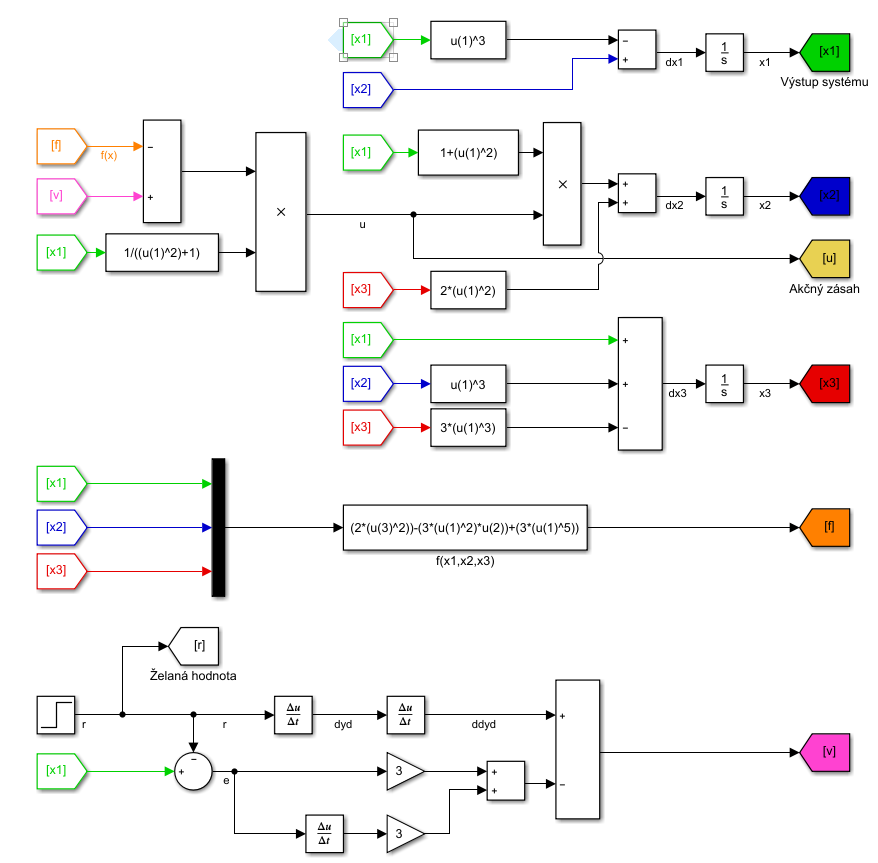
\includegraphics[width=\linewidth]{sysPr2complet}
		\caption{Kompletná schéma riadného systému pomocou nelineárneho riadenia.}
		\label{fig:svlvvPr2All}
	\end{figure}
	\subsubsection{Návrh PID}		
	Pre porovnanie skúsme navrhnúť ešte PID regulátor pre systém linearizovaný v rovnovážnom bode $x_1 = x_2 = x_3 = 0$. Po linearizovaní bude mať systém tvar \cref{eqn:svlvvPr2LinearizSys}. 
	\begin{equation}
	\begin{aligned}
	\Delta \dot{x_1}  &= \Delta x_2 \\
	\Delta \dot{x_2} &= \Delta u \\
	\Delta \dot{x_3} &= \Delta x_1 \\
	\Delta y &= \Delta  x_1
	\end{aligned}
	\label{eqn:svlvvPr2LinearizSys}
	\end{equation}	
	Pre jednoduchší návrh parametrov regulátora si vyjadríme prenosovú funkciu systému. Vyjadrenie je ukázané v \cref{eqn:svlvvPr2Prenos}. V tomto momente ešte potrebujeme zapojiť pred systém regulátor a vyjadriť prenos uzavretého regulačného obvodu.
	\begin{equation}
	\begin{aligned}
	\Delta  y &= \Delta x_1 = \frac{1}{s}  \Delta x_2 = \frac{1}{s^2}  \Delta u \\
	\implies \frac{\Delta y}{\Delta u } &= \frac{1}{s^2} \\
	\end{aligned}
	\label{eqn:svlvvPr2Prenos}
	\end{equation}
	Zapojíme na vstup systému PID regulátor, ako je na \cref{fig:svlvvPr2ZapPID}. Ktorý má prenos \cref{eqn:svlvvPr2PIDPrenos}, kde $P, D, I$ sú parametre regulátora. Pre zjednodušenie, prenosy systému a regulátora roznásobíme a dostaneme tak prenos otvoreného obvodu $G_{ORO}$ daný \cref{eqn:svlvvPr2PIDPrenosORO}. 
	\begin{figure}[h!]
		\centering
		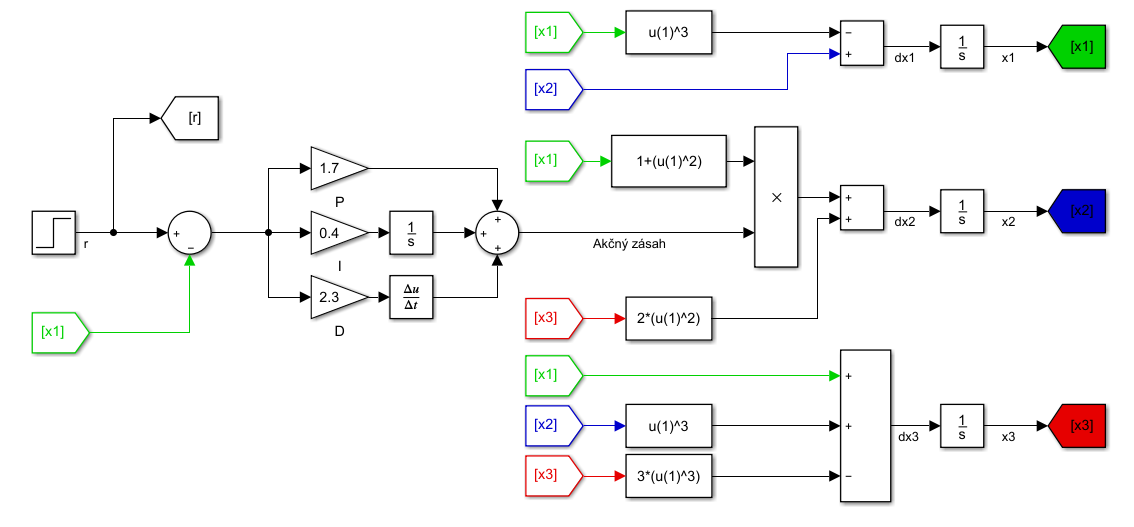
\includegraphics[width=0.8\linewidth]{svlvvPr2ZapPID}
		\caption{Zapojenie PID regulátora}
		\label{fig:svlvvPr2ZapPID}
	\end{figure}
	\begin{equation}
		\begin{aligned}
		\frac{U(s)}{E(s)} = P + Ds + \frac{I}{s} \\
		\end{aligned}
		\label{eqn:svlvvPr2PIDPrenos}
	\end{equation}
	\begin{equation}
		\begin{aligned}
		G_{ORO} = \frac{Ps + Ds^2 + I}{s^3} \\
		\end{aligned}
		\label{eqn:svlvvPr2PIDPrenosORO}
	\end{equation}
		Vyjadríme prenos uzavretého regulačného obvodu $G_{URO}$ podľa pravidla zápornej spätnej väzby \cref{eqn:svlvvPr2Pravidlo}. Dostaneme tak prenos \cref{eqn:svlvvPr2PrenosURO}.
	\begin{equation}
		\begin{aligned}
		G_{URO} = \frac{G_{ORO}}{1 + G_{ORO}}
		\end{aligned}
		\label{eqn:svlvvPr2Pravidlo}
	\end{equation}
	\begin{equation}
		\begin{aligned}
		G_{URO} &= \frac{\frac{Ps + Ds^2 + I}{s^3}}{1 + \frac{Ps + Ds^2 + I}{s^3}}  \\
		&= \frac{Ps + Ds^2 + I}{s^3 + Ps + Ds^2 +I}
		\end{aligned}
		\label{eqn:svlvvPr2PrenosURO}
	\end{equation}
	
	Využijeme metódu Pole-Placement na návrh parametrov regulátora, umiestnime póly na nasledovných pozíciách komplexnej roviny $p_1 = -1, p_2 = -0.8, p_3 = -0.5$. Teda nech sú póly reálne a záporné, čo zabezpečí stabilitu lineárneho systému, keďže na kvalitu riadenia zatiaľ nekladieme dôraz.
	
	Polynóm, ktorý bude mať zvolené korene, získame roznásobením polynómov prvého stupňa, ktorých korene sú zvolené póly ( \cref{eqn:svlvvPr2ZiadanPoly}). 
	\begin{equation}
		\begin{aligned}
		P(s) &= (s - p_1)(s - p_2)(s - p_3) \\
		&= (s + 1)(s + 0.8)(s + 0.5) \\
		&= s^3 + 2.3s^2 + 1.7s + 0.4\\
	\end{aligned}
	\label{eqn:svlvvPr2ZiadanPoly}
	\end{equation}
	Tento želaný polynóm porovnáme s charakteristickým polynómom URO, teda \cref{eqn:svlvvPr2Porovnanie}, dostaneme tak rovnice \cref{eqn:svlvvPr2RovniceParametrovPID} z ktorých vypočítame parametre regulátora.
	\begin{equation}
		\begin{aligned}
			s^3 + 2.3s^2 + 1.7s + 0.4= s^3 + Ps + Ds^2 + I\\
		\end{aligned}
		\label{eqn:svlvvPr2Porovnanie}
	\end{equation}
	\begin{equation}
		\begin{aligned}
		\begin{matrix}
			P &= 1.7 \\
			D &= 2.3 \\ 
			I &= 0.4 \\
		\end{matrix}
		\label{eqn:svlvvPr2RovniceParametrovPID}
		\end{aligned}
	\end{equation}
	Aplikujme PID regulátor na nelineárny systém (\cref{fig:svlvvPr2ZapPID}), ktorý chceme riadiť . Výsledok zo simulácie je na \cref{fig:svlvvPr2VysPID}.	
	
	\subsubsection{Porovnanie riadenia}	
	\begin{figure}[h!]
		\centering
		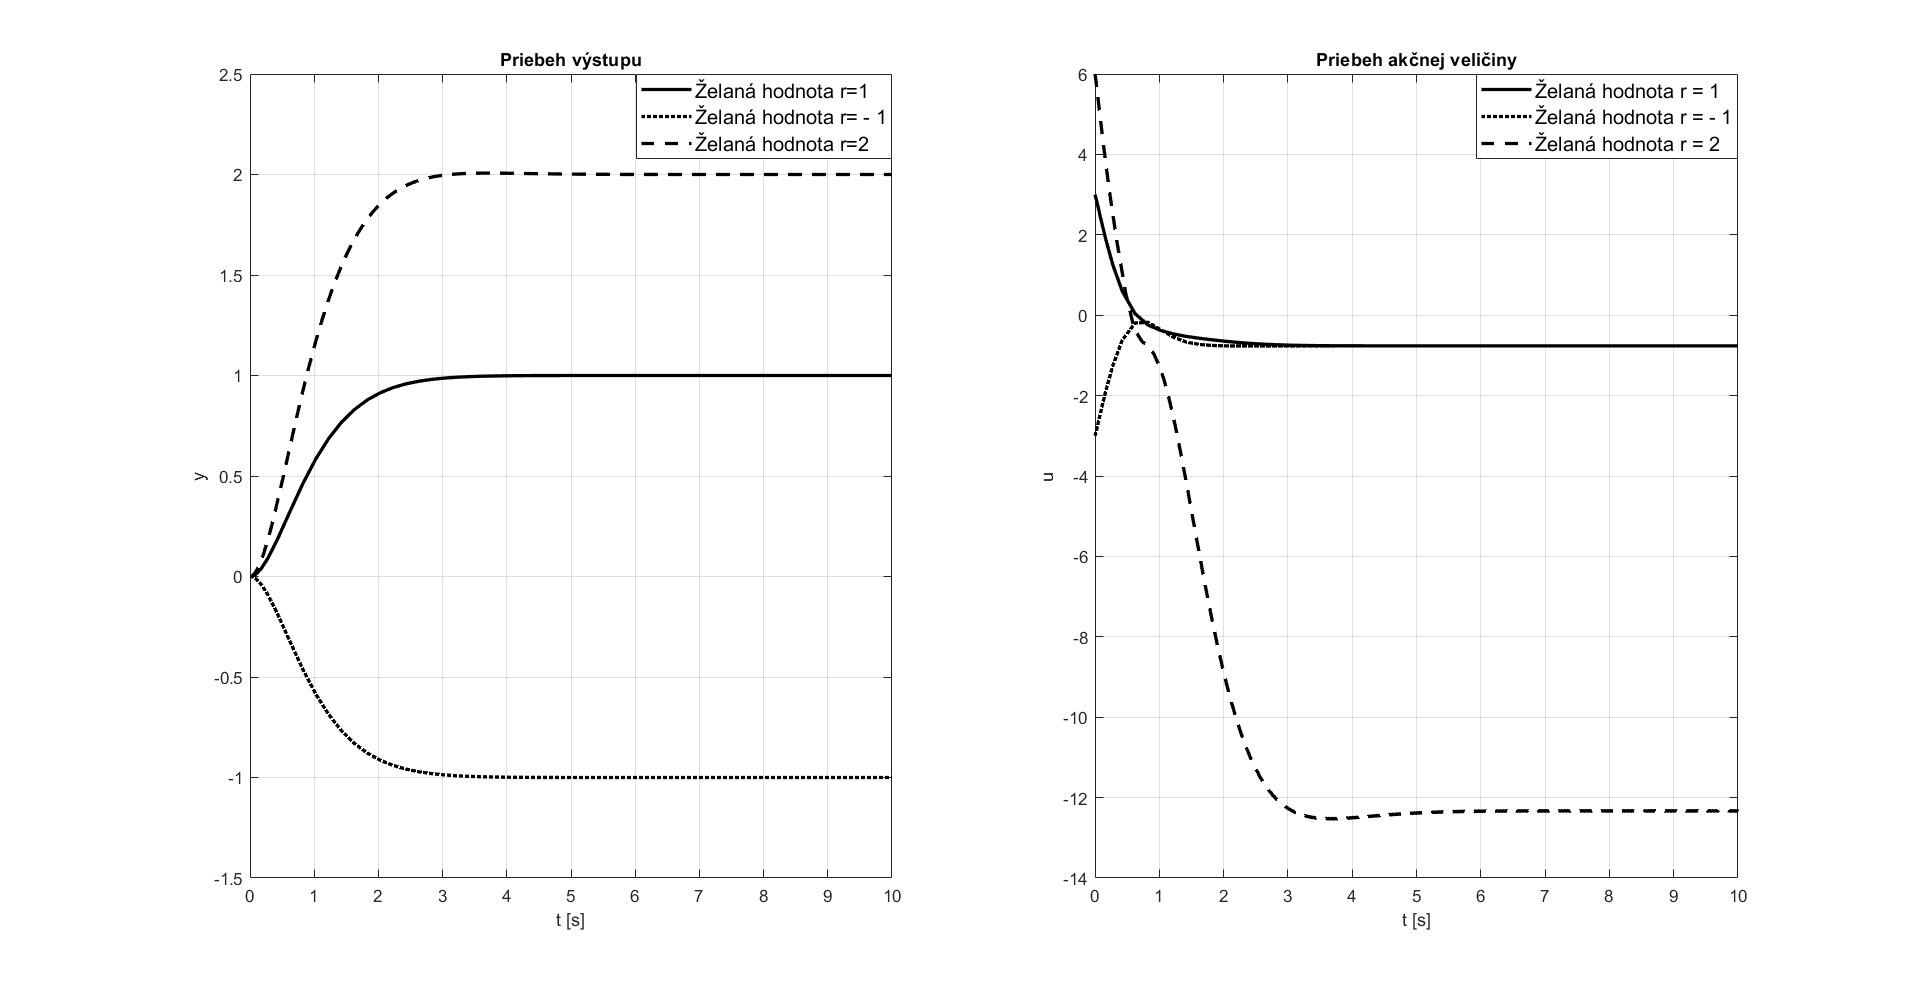
\includegraphics[width=\linewidth]{pr2vys}
		\caption{Regulácia výstupu na konštantnú hodnotu nelin. regulátorom navrhnutým pomocou metódy spätnoväzbovej linearizácie vstupno-výstupnej.}
		\label{fig:svlvvPr2Vys}
	\end{figure}
	\begin{figure}[h!]
		\centering
		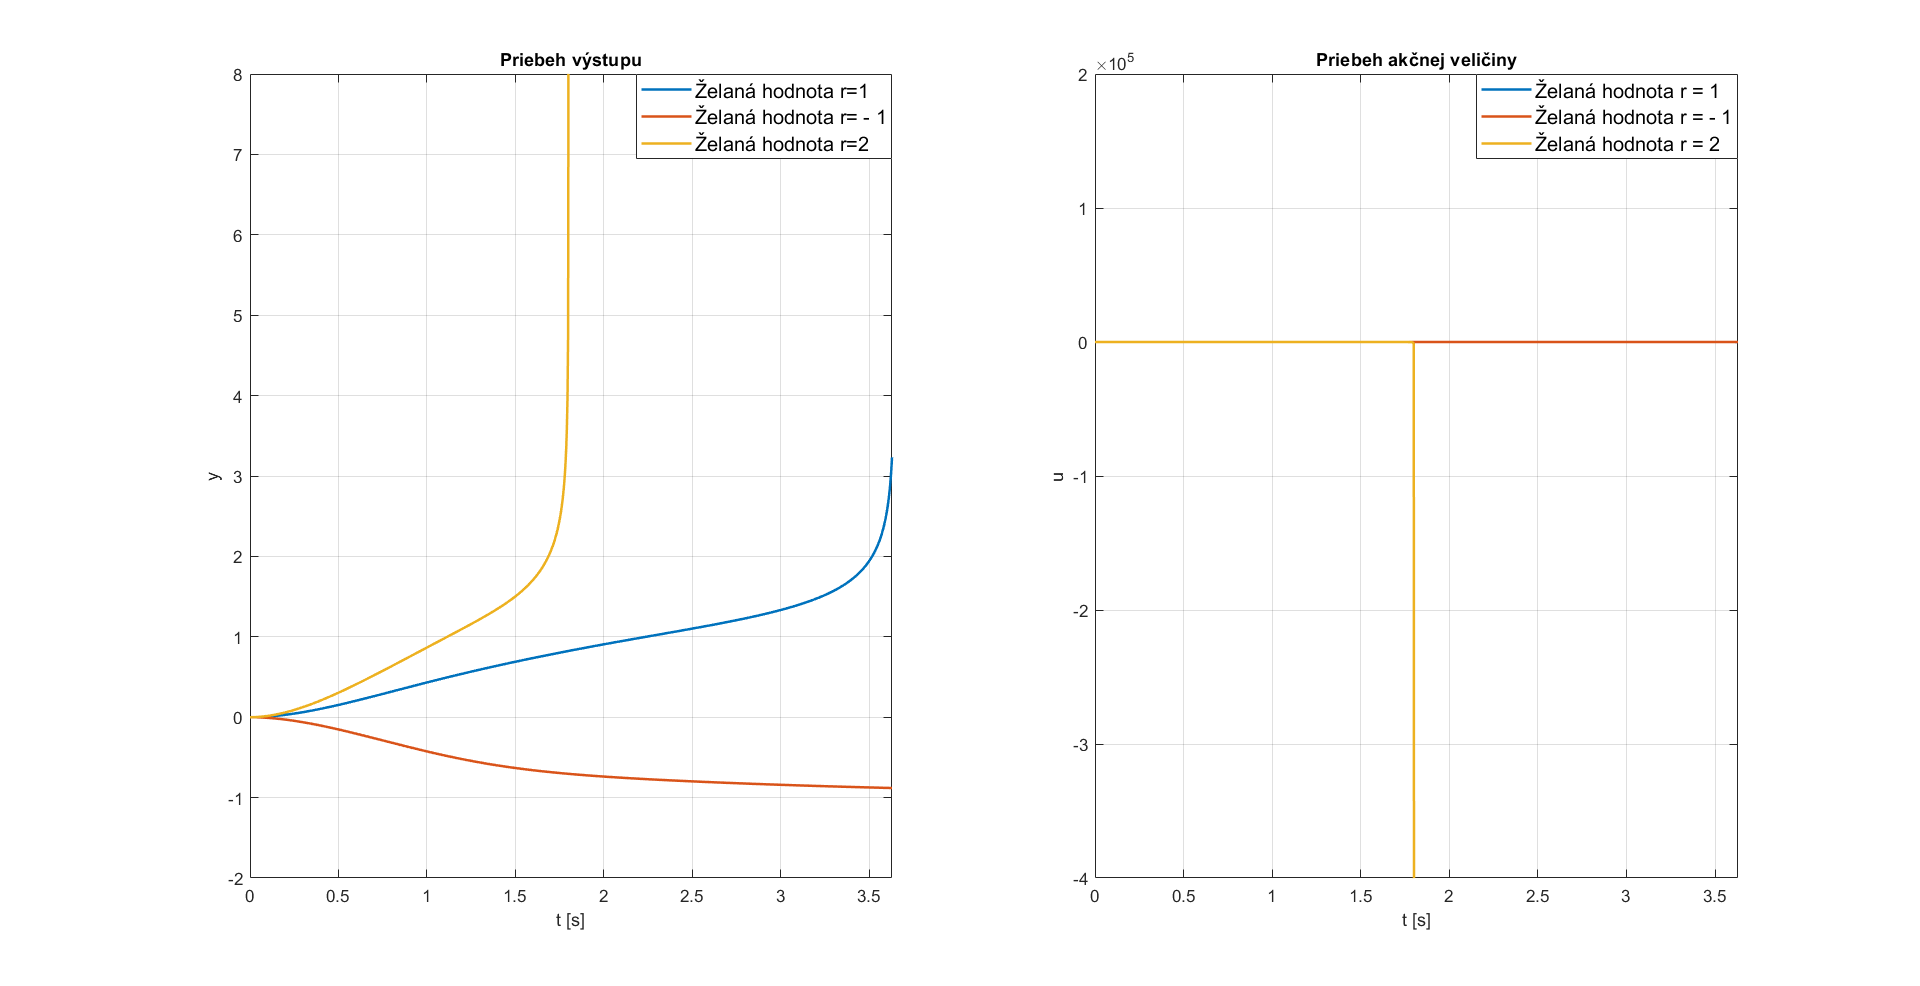
\includegraphics[width=\linewidth]{pr2vysPID}
		\caption{Regulácia výstupu na konštantnú hodnotu PID regulátorom navrhnutým pomocou metódy pole-placement}
		\label{fig:svlvvPr2VysPID}
	\end{figure}
	\newpage
	\subsubsection{Záver}
	Z výsledku môžeme usúdiť, že nelineárne riadenie je v tomto prípade, nevyhnutné. Systém regulovaný PID regulátorom nebol schopný sa stabilizovať v takom okolí pracovného bodu ako to dokázal systém s regulátorom navrhnutým pomocou metódy vstupno-výstupnej spätnoväzbovej linearizácie. 
\end{document}
